\chapter{Software}\label{cha:appendix2}


\section{Open-Source Thesis}
All \LaTeX files, data and code used to build the figures in this thesis are available on GitHub.

The code can be found here:\newline \url{https://github.com/johann997/QDEV_masters_thesis}.

\section{Data Acquisition and Analysis}

I was fortunate to join FolkLab after Timothy Child had largely rewritten and significantly improved the acquisition code. However, code is never in a final state, and over the years, I contributed to the repository with new scan functions, analysis, and function dependency visualisation.

The code can be found here:\newline 
\url{https://github.com/folk-lab/IgorAcq}



For analysis, I built upon some initial code provided by Josh and Silvia. Currently, the code used to fit data to NRG lives in a separate repository from the acquisition code. 

The code can be found here:\newline \url{https://github.com/johann997/KondoConductanceAnalysis}

\section{Device Simulation}

The code can be found here:\newline \url{https://github.com/johann997/2deg_yodels}


\begin{figure}[!bht]
 \begin{center}
%% includegraphics: comment the following if not using the graphicx package
 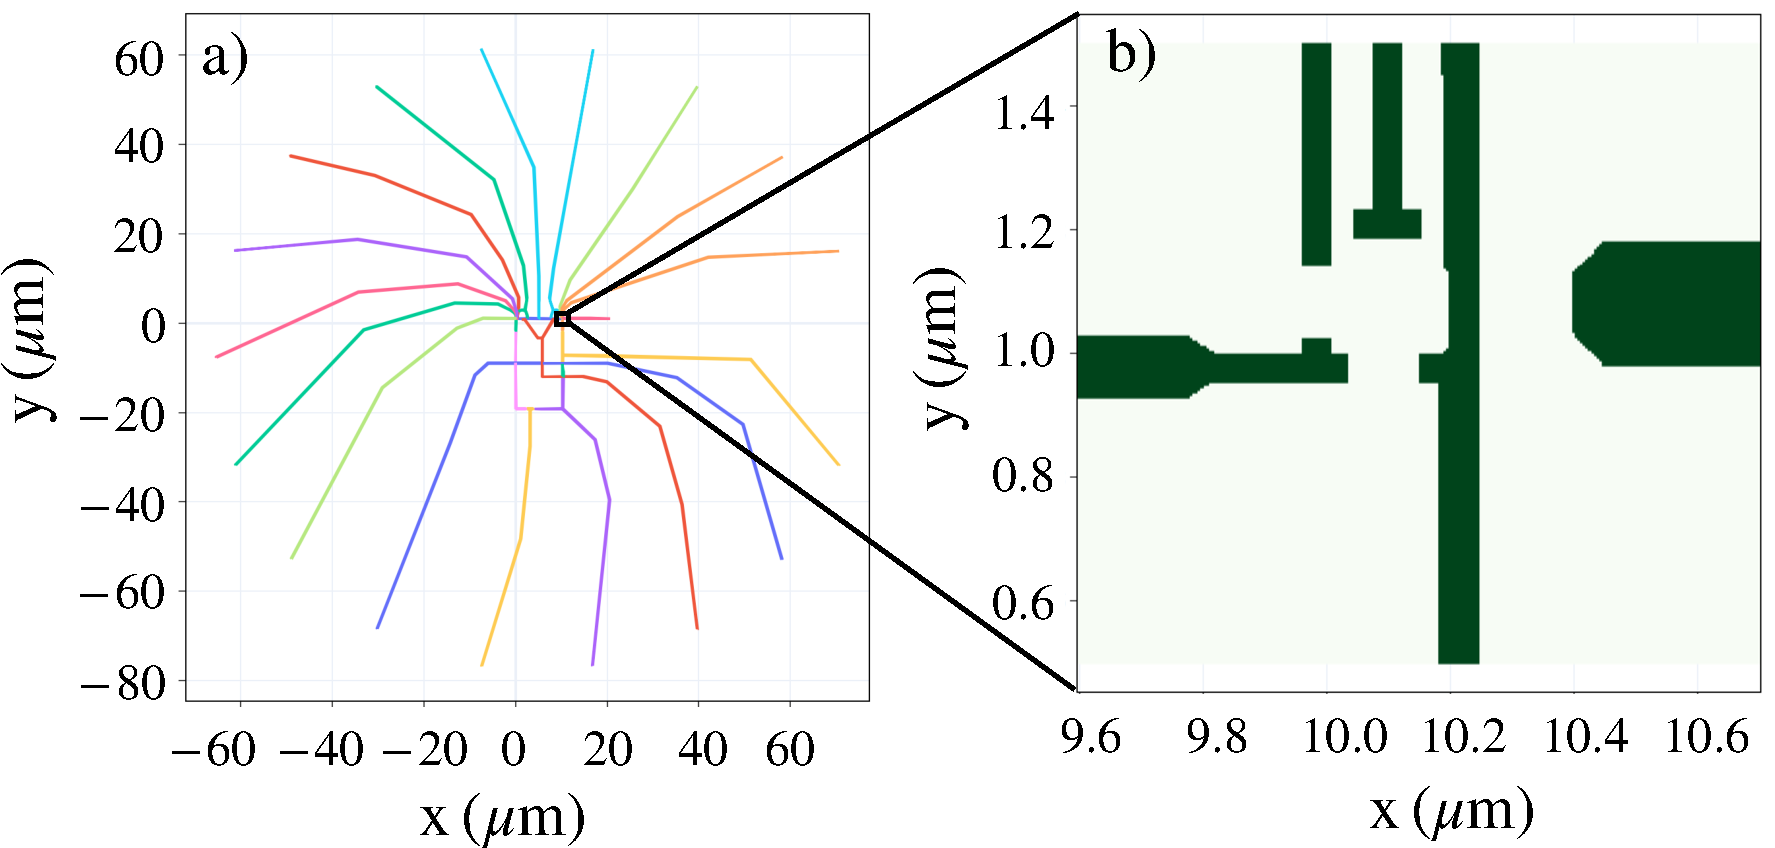
\includegraphics[width=1.0\textwidth]{figures/appendix/appendix2_load.pdf}
 \caption[Loading a DXF Design File]{\label{fig:appx/kwant_load} 
 (\textbf{a}) Plot of the uploaded .dxf. Each polyline in the .dxf is saved as a new trace (hence, the varying colours). (\textbf{b}) Discretised matrix from a zoom in on the uploaded design file. The matrix was defined by specifying the min, max and x, y coordinates and the number of points to discretise in the x and y direction (here numptsy and numptsy = 250). This approach is quite rudimentary and not optimised, but is sufficient at capturing the device design geometry.}
 \end{center}
\end{figure}



Fabrication and measurement of quantum devices can be costly and time-consuming. As part of a class project, I developed an easy-to-install, open-source application that allows users to upload a .dxf file and calculate the electric potential from user-determined gate voltages.
\textsc{kwant}~\cite{kwant} is used to calculate transport properties by applying a tight-binding approximation. A tight-binding model reduces computation so that users can simulate pinch-off or charge stability diagrams in `real time'. This app aids the design process by providing quick, semi-quantitative information on design choices. 




For user convenience, drag-and-drop functionality is used. Upon uploading the .dxf file, \textsc{ezdxf} Python library is used to extract the polylines. Users specify device areas by defining min, max and x, y coordinates, and point discretisation (Fig.~\ref{fig:appx/kwant_load}). 


\begin{figure}[!bht]
 \begin{center}
%% includegraphics: comment the following if not using the graphicx package
 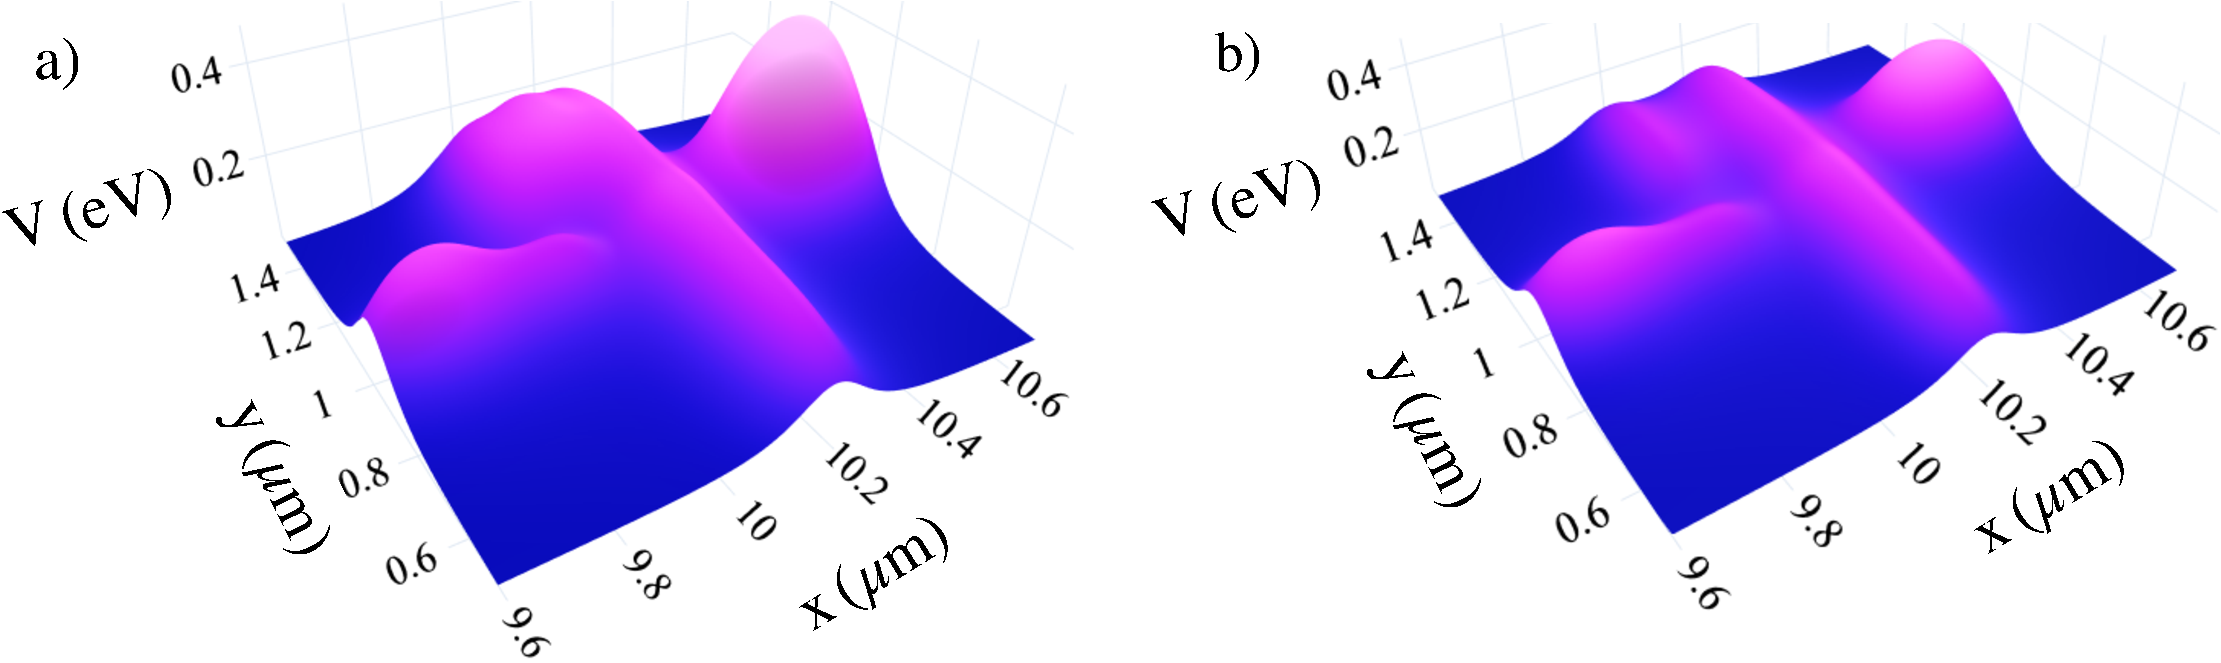
\includegraphics[width=1.0\textwidth]{figures/appendix/appendix2_potential.pdf}
 \caption[Electric Potential Calculation]{\label{fig:appx/kwant_pot} 
 (\textbf{a}) 3d map of the electrostatic potential landscape $90\,\mathrm{nm}$ below the surface of the heterostructure, calculated using the bare potentials on the gates on top of the heterostructure. (\textbf{b}) Varied potential landscape by changing the voltages on the gates.}
 \end{center}
\end{figure}



The electric potential is calculated using the method developed by Davies~\cite{Davies1995}. This method offers the advantage of computational efficiency. A single `geometric factor' is initially calculated and the resulting potential is simply the product of the geometric factor with the gate voltages. Real-time updates of the plotted potential are achieved using sliders (Fig.~\ref{fig:appx/kwant_pot}). The disadvantage of this method is that screening terms are not included, and hence, the calculation can only be used as a qualitative visualisation of the electric potential profile.




\begin{figure}[!bht]
 \begin{center}
%% includegraphics: comment the following if not using the graphicx package
 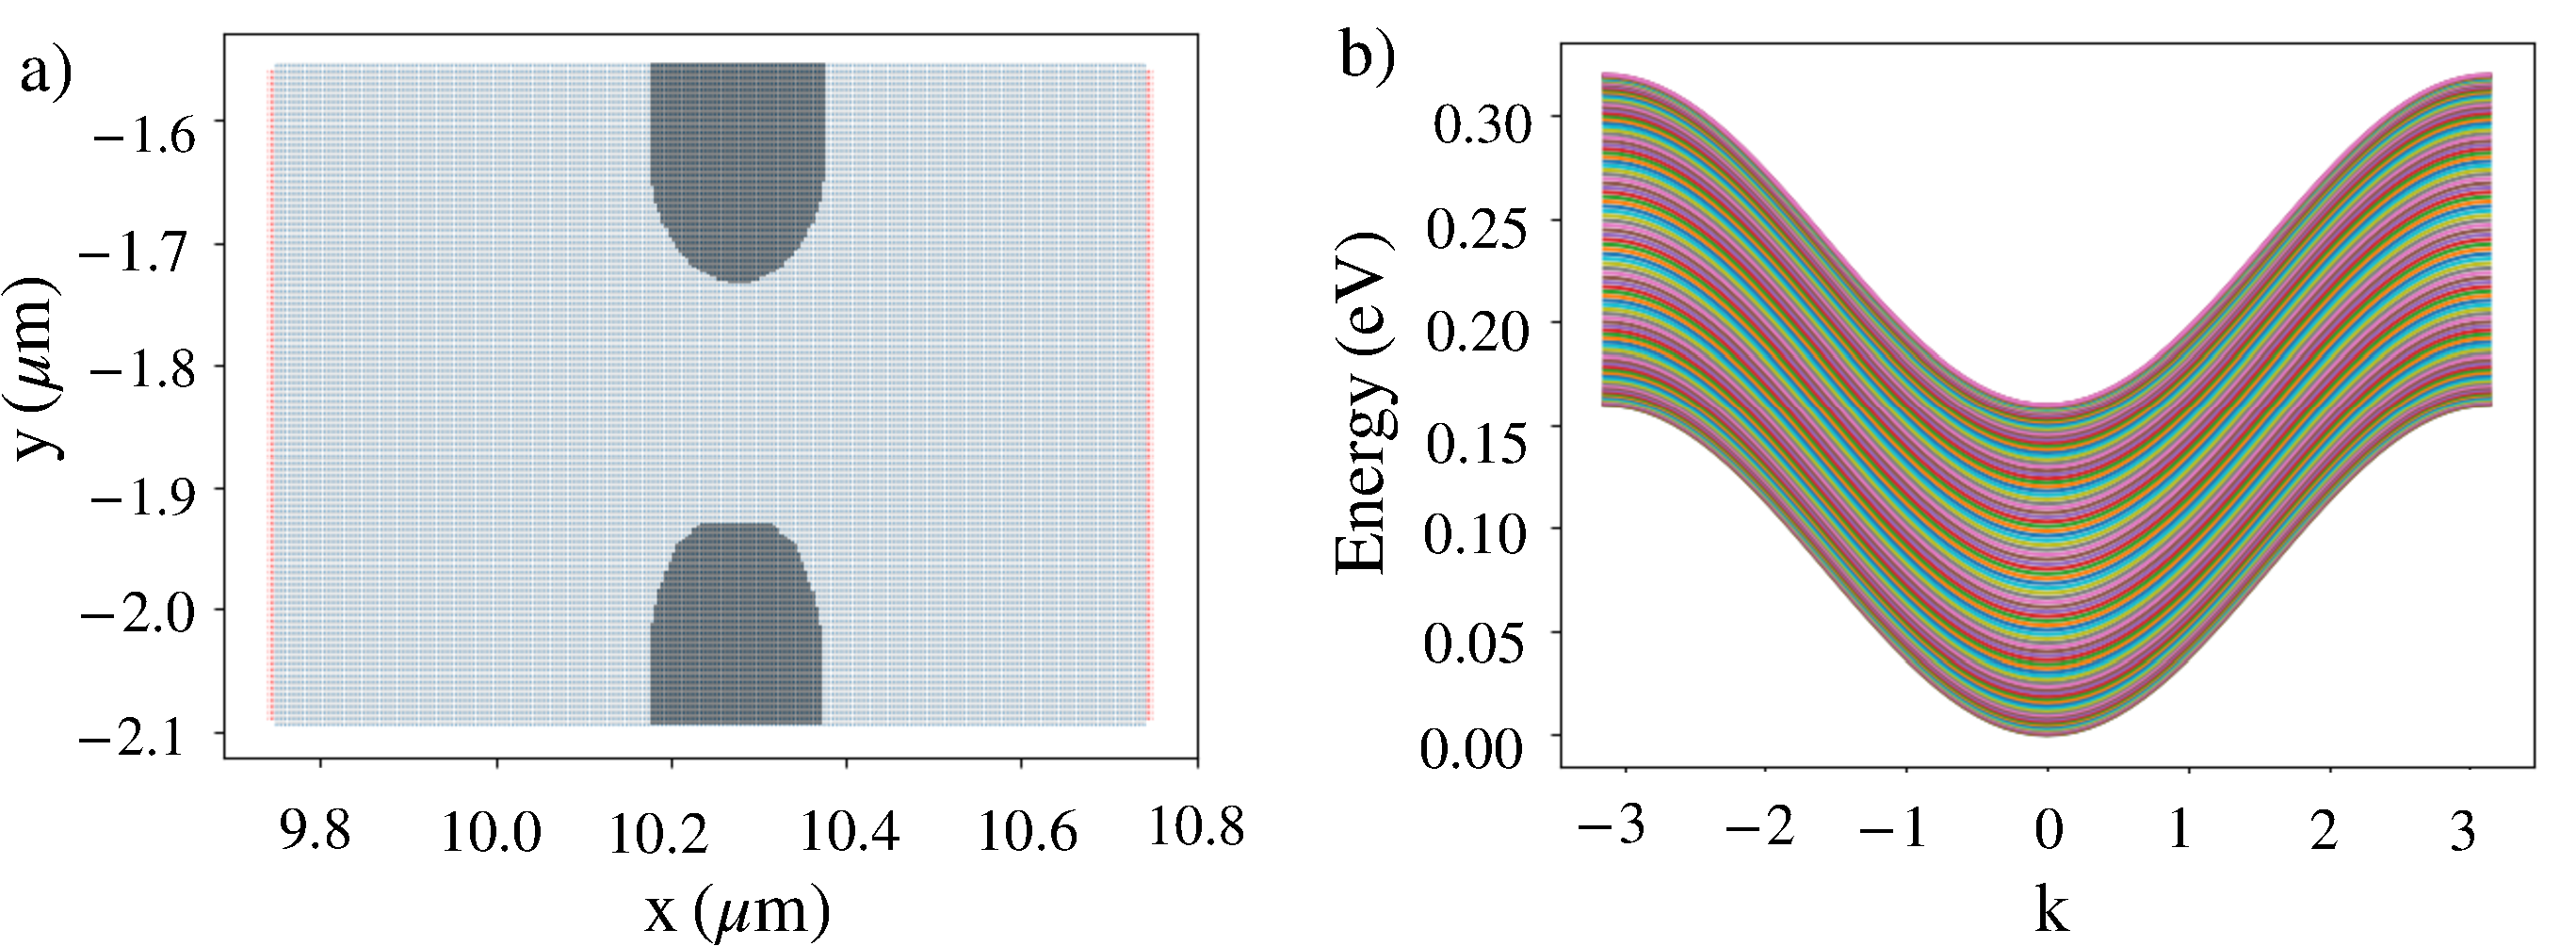
\includegraphics[width=1.0\textwidth]{figures/appendix/appendix2_kwant.pdf}
 \caption[\textsc{kwant} : Tight Binding Model and Band Structure]{\label{fig:appx/kwant_tightbind} 
 (\textbf{a}) Gate design of a QPC on top of the \textsc{kwant}~\cite{kwant}, tight binding system. A square lattice with lattice constant $5\,\mathrm{nm}$ is chosen. The infinite leads are shown in red on the left and right axes. (\textbf{b}) Band structure calculation of this tight binding system. The user can calculate transport properties at the different allowed energy levels in the band structure.}
 \end{center}
\end{figure}





\textsc{kwant} is utilised to build a tight-binding model which can be solved to provide access to transport properties~\cite{kwant}. This method assumes electrons are tightly bound to their respective atoms, with interactions from neighbouring atoms considered as perturbations. A \textsc{kwant} system comprises a finite scattering region described by a scattering Hamiltonian $H_S$ and infinite regions called leads (these represent the ohmic contacts in an experiment).


\begin{figure}[!bht]
 \begin{center}
%% includegraphics: comment the following if not using the graphicx package
 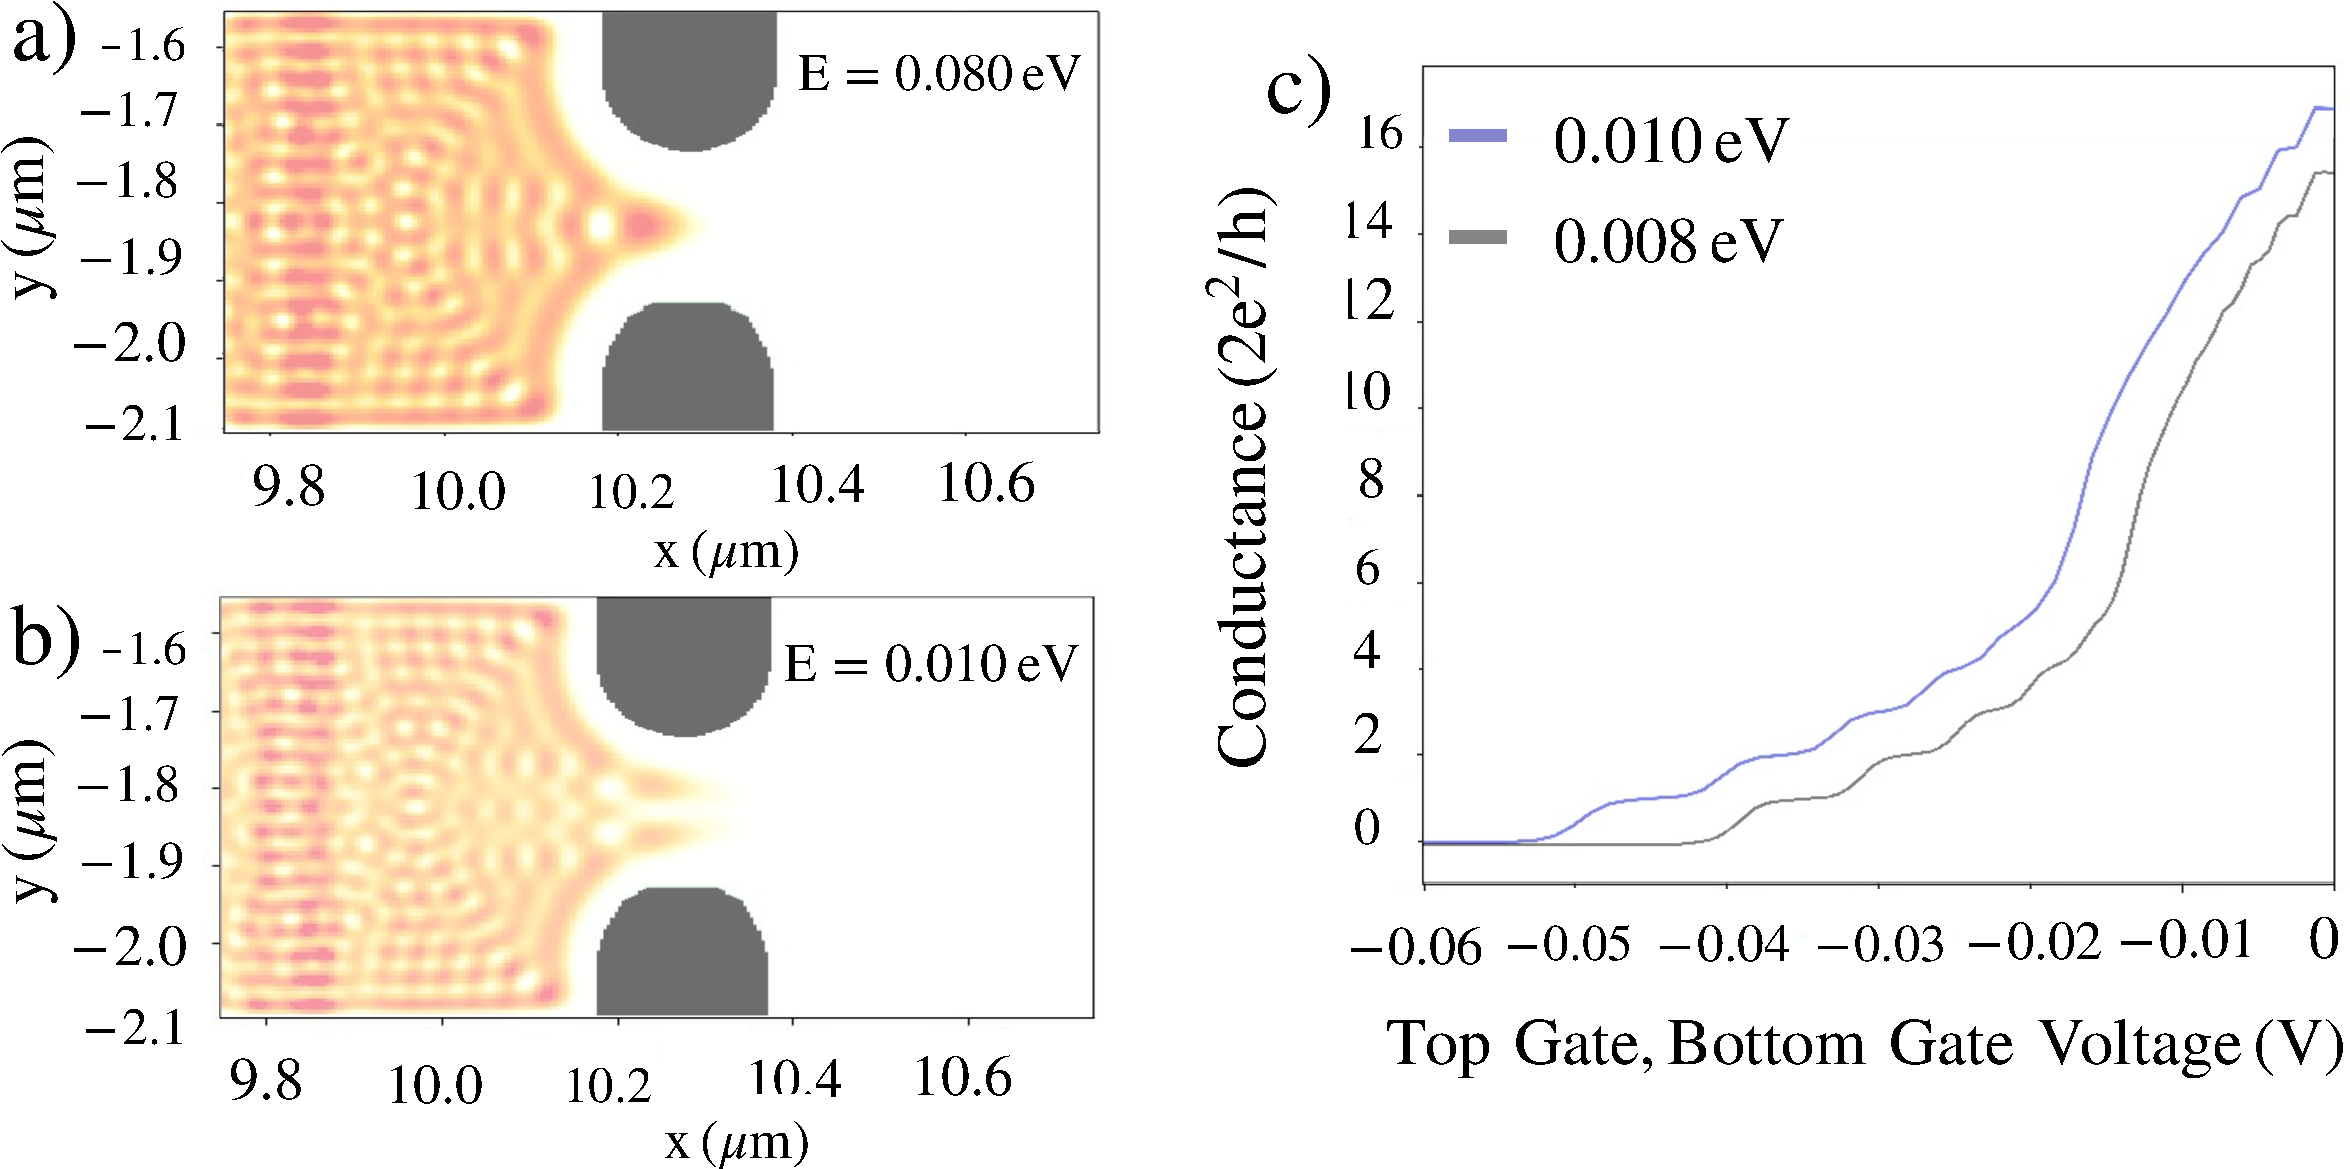
\includegraphics[width=1.0\textwidth]{figures/appendix/appendix2_wavefunction.pdf}
 \caption[\textsc{kwant} : Transport Simulation]{\label{fig:appx/kwant_transport} 
 (\textbf{a}) Calculated wavefunction squared at lower band energy such that a single channel propagates through the QPC. (\textbf{b}) Calculated wavefunction squared at increased band energy so that two channels propagate through the QPC. (\textbf{c}) Calculated conductance through the QPC at two energy bands as the voltage on both QPC gates is varied. Conductance drops to zero at lower gate potentials. Both curves show the characteristic QPC conductance plateaus at integer multiples of $\mathrm{2e^2/h}$. }
 \end{center}
\end{figure}


In the app, the \textsc{kwant} system is generated by defining the lattice constant and lead locations. A plot of the system is shown in Fig.~\ref{fig:appx/kwant_tightbind}\textbf{a} and corresponding band structure in Fig.~\ref{fig:appx/kwant_tightbind}\textbf{b}. An energy level is selected to compute transport properties.
A plot of the wavefunction squared is shown in Fig.~\ref{fig:appx/kwant_transport}\textbf{a}, where a single channel is shown to propagate through the QPC. 
The calculated conductance at varying gate potentials is shown in Fig.~\ref{fig:appx/kwant_transport}\textbf{c}, where the characteristic QPC conductance plateaus at integer multiples of $\mathrm{2e^2/h}$ are found. 



